\section{Background and Design Considerations}
\label{sect:background}

Figure~\ref{fig:collocated} illustrates a converged IaaS cloud architecture 
where
each commodity server hosts a number of virtual machines and storage of these servers
is clustered using a distributed file system~\cite{googlefs03,hdfs10,NutanixPaper}.
Each physical machine hosts multiple virtual machines.  Every virtual machine
runs its own guest operating system and accesses virtual hard disks 
stored as image files maintained by the operating system running on the
physical host.
For VM snapshot backup, file-level semantics are normally not provided.
Snapshot operations take place at the virtual device driver level, which
means no fine-grained file system metadata can be used to determine the changed data. 
%This architecture does not use a separate  backup facility for a lower cost and 
%reduces the network bandwidth consumption in transferring the raw data for backup. 
%A backup service may co-locate with other cloud services on these commodity servers and 
%stores deduplicated data  in  the storage in this cluster or in
%a separate storage cluster.


%runs a backup service and 


%As discussed earlier, co-locating a backup service on the existing
%cloud cluster avoids the extra cost to acquire a dedicated backup facility

\begin{figure}[htb]
    \centering
    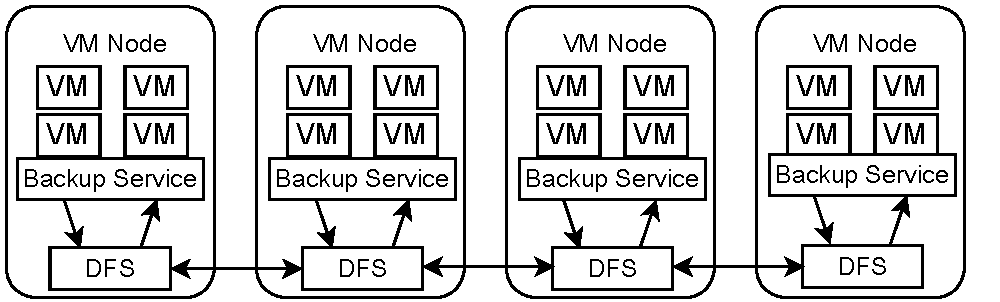
\includegraphics[width=3in]{images/colocated-arch}
    \caption{VM snapshot backup running on a converged cloud cluster.}
    \label{fig:collocated}
\end{figure}

File backup systems have been developed to use fingerprints generated for
data ``chunks''  to identify duplicate
content~\cite{venti02,Rhea2008}.  In a simple implementation,
it is expensive to compare a large number of 
fingerprints
so several techniques have been proposed to improve duplicate identification. 
For example, the data domain method ~\cite{bottleneck08} 
uses  an in-memory Bloom filter and a prefetching cache for data chunks 
which may be
accessed.  
%An improvement to this work with parallelization is in ~\cite{MAD210,DEBAR}.
Approximation techniques are studied in~\cite{extreme_binning09,Guo2011,WeiZhangIEEE}  
to reduce memory requirements at the cost of some loss of deduplication
efficiency.
Additional inline deduplication techniques are studied in ~\cite{sparseindex09,Guo2011,Srinivasan2012}
and a parallel batch solution for cluster-based deduplication is 
studied in ~\cite{wei2013}. 
All of the above approaches have focused on optimization of deduplication
efficiency or speed, and none of them have considered the impact
of deduplication on fault resilience in a cloud environment.  To do so, we
examine the following properties of VM snapshot deduplication for converged
IaaS architectures.
%considered in this paper.
%Our consideration is discussed below.
%VM dependence minimization during deduplication and file system block management.
\paragraph*{Local versus Global Deduplication} --
If deduplication is implemented strictly in the storage system,
a data chunk is compared with fingerprints collected from all VMs during
the deduplication process, and only a small number of
copies of duplicates are stored in the storage.  This sharing
artificially creates hidden data dependencies among different VMs owned by
different 
who
contract for isolation 
by the IaaS cloud platform.  That is, the unit of failure visible to the cloud
user is the VM, but the unit of sharing in a deduplicated data store is the
data chunk. 

%Further, 
%this artificial dependence affects fault isolation since 
%the loss of all replicas of a data chunk can affect the otherwise unrelated
%VMs that share it.  

Indeed, the greater the deduplication efficiency, the less
the data redundancy is maintained, and the greater the ``hidden'' data
dependence between VMs that must be hosted as if they were physically isolated.
%machine failures happen periodically 
%in a large-scale cloud and
%loss of a small number of shared data chunks can 
%cause the unavailability of snapshots for a large number of virtual machines.
Thus,
restricting deduplication to be local to each VM (but across snapshots) 
aligns the units of storage with the isolation properties guaranteed by the
cloud at the possible expense of storage efficiency.
%Localizing the impact of deduplication can increase fault isolation and resilience.
%Thus from the fault tolerance point of view,  duplicate sharing among multiple VMs is 
%discouraged. 

Additionally, storage efficient deduplication can be computationally expensive
to implement in a distributed setting.  In particular, duplicate detection is
logically a ``global'' operation over all data chunks
under consideration.
By localizing duplicate search, the computational requirements
for deduplication can be reduced, because fewer chunks must be compared.
Further, deduplication of VMs can easily be implemented in
parallel.
 
Another disadvantage of cross-VM sharing is that it complicates 
snapshot deletion, 
which occurs frequently when snapshots expire regularly. 
The mark-and-sweep approach~\cite{Guo2011,Fabiano2013}  is effective for
deletion, but still carries a significant cost, especially in the distributed cloud
setting.
%to count if a data chunk is still shared by other snapshots. 

Thus,
localizing deduplication to the VM can align fault isolation properties and
guarantees, improve the computational efficiency of snapshot maintenance, and
simplify snapshot deletion over non-localized approaches at the possible
expense of storage efficiency.

%minimize data sharing and simplify deletion while sacrificing 
%deduplication efficiency, and  can facilitate parallel execution of snapshot operations.
\paragraph*{Units of Storage versus Units of Sharing} --
The file system block  size in a distributed file system such as  
the Hadoop file system and the Google file system~\cite{googlefs03}
is large (e.g.  64MB) so as to optimize file system performance
for big data.
Typically, deduplication implementations use smaller block sizes (4K bytes to
8K bytes on average~\cite{Jin2009}).
In addition to the failure correlation that cross-VM data deduplication can
introduce, disk block sharing of data chunks is another potential source of
hidden data dependence.
Thus a VM-centric solution should consider how data chunks from VMs are
distributed among large file system blocks when a large-scale distributed file
system is used for snapshot storage.

%a minimum association of FSBs to VMs in the packaging
%process. By minimizing this association we can improve fault tolerance by
%reducing the number of VMs affected when storage nodes are lost.
 

\paragraph*{Moderating Resource Usage} --
In a converged setting, the resources that are used to implement snapshot
backup and deduplication are the same resources that must support cloud-hosted
VMs.  Thus the backup service must share the resources available to
other cloud services as illustrated in Figure~\ref{fig:collocated},
and has to minimize its impact on user-deliverable performance.
%The key resource for global comparison  is memory for storing the fingerprints.
%During snapshot deletion, reference counting for all unique blocks used in all VMs requires a significant resource usage
%too.  Thus we seek for the low-profile techniques with approximation and low resource consumption. 

For the remainder of this paper, 
we term the traditional deduplication approach {\em VM-oblivious} (VO)
because it manages duplicate data chunks without consideration of VMs.
With the above  considerations in mind, we propose a 
VM-centric approach (called VC)
for a co-located backup service that has a resource usage profile
suitable for use with converged cloud architectures.  

In designing a VC deduplication solution, we have considered and adopted some of
the following previously-developed techniques.
\begin{itemize}
\item {\em Changed Block Tracking} --
VM snapshots can be  backed up  incrementally by identifying data segments that have
changed from the previous version of the snapshot~\cite{Clements2009,Vrable2009,TanIPDPS2011}.
Such a scheme  is  VM-centric since deduplication is localized to the snapshot
history for each VM.
%We are seeking for a tradeoff since 
%global signature comparison can deliver additional compression~\cite{Guo2011,Dong2011,extreme_binning09}.
\item {\em Stateless  Data Routing} --
One approach to scalable duplicate comparison is to use a content-based hash
partitioning algorithm called stateless data routing by Dong et al.~\cite{Dong2011}.
Stateless data routing divides the deduplication work with a similarity approximation. This work 
is similar to Extreme Binning by Bhagwat et al.~\cite{extreme_binning09} and 
each request is routed  to a machine which holds
a Bloom filter  or can fetch on-disk index for additional comparison.
While this approach is VM-oblivious, it motivates us to  use  a combined signature of a dataset to narrow
VM-specific local search.
\item {\em Sampled Index for Memory Parsimony} -- 
One effective approach that reduces memory usage is 
to use a sampled index with prefetching, proposed  by Guo and Efstathopoulos\cite{Guo2011}. 
The algorithm is VM oblivious and it is not easy  to adopt for a distributed architecture. 
To use a distributed memory version of the sampled index, every deduplication request
may access a remote machine for index lookup and the overall overhead of access latency for all requests
can be significant.  
\end{itemize}

We will first discuss and analyze the integration of the VM-centric deduplication strategies with fault isolation 
and discuss snapshot deletion support, then present an implementation design. 
